Figure \ref{RigtBillede} shows a Rich picture. This rich picture gives an overview of the users situation from the viewers position.
The symbols represent different units, processes and problems.
To begin with there will be looked upon the symbols and they will be explained. Afterwards the situation will be explained in depth.

  \begin{figure}[H]
	\centering
	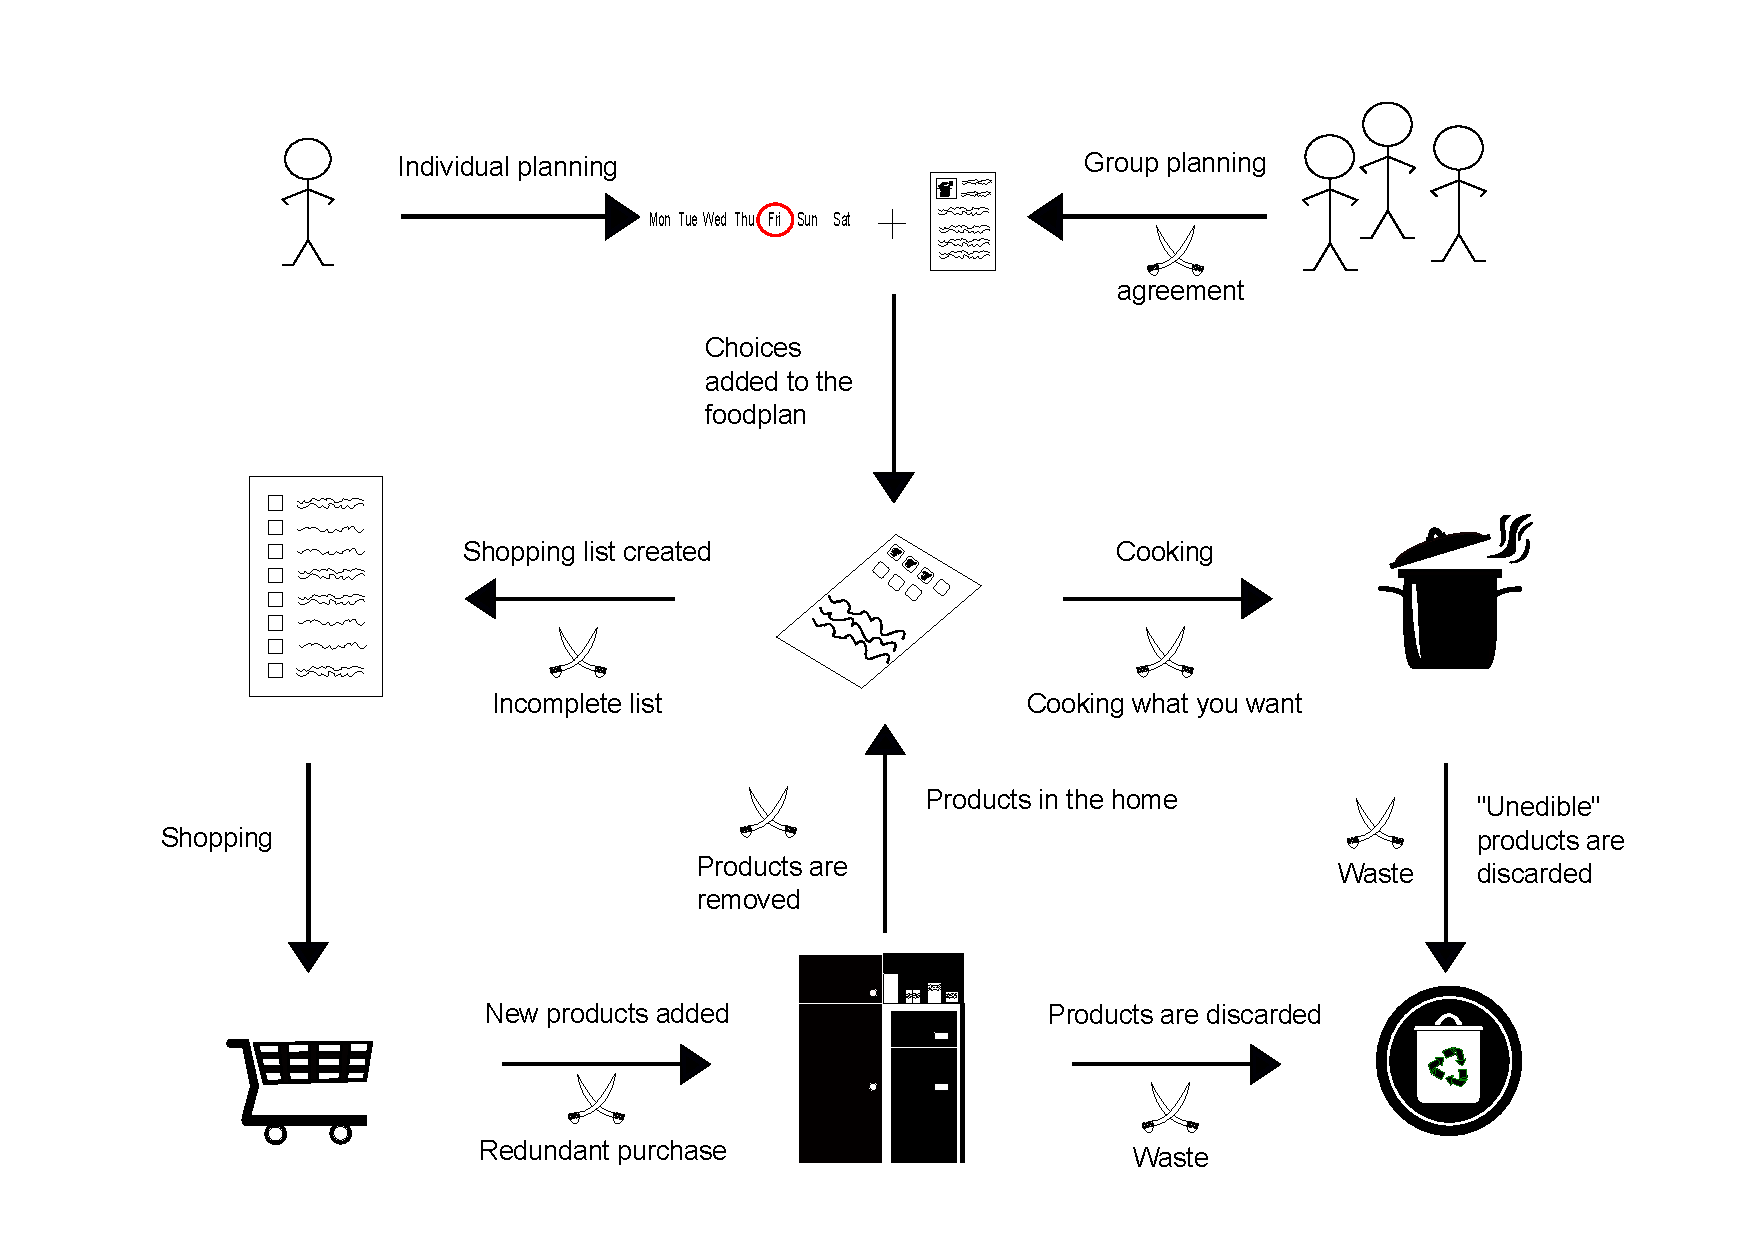
\includegraphics[width=1.00\textwidth]{Grafik/FoodPlanner/InkscapeTegninger/RigtBillede.pdf}
	\caption{A rich picture of the user's situation from the viewers position}
	\label{RigtBillede}
\end{figure}
\fxnote{resize elementer så de er lige store + kosmetiske fejl}
\textbf{Units} includes people, physical objects, organizations and roles.
\begin{itemize}
  \item On the top line the stick man symbol is used to represent a user and to the top right there is the group of users symbol. 
  \item On the middle line is the overview of the food plan symbol and shopping list symbol which is used to depict the users overview of the two units. 
  \item On the bottom line is the inventory symbol used to depict the household's storage of food products and the trashcan symbol.    
\end{itemize}
\textbf{Processes} includes different categories such as work and production, planning and control and information treatment. In Figure \ref{RigtBillede} all of the arrows between the symbols signifies different processes.
\begin{itemize}
\item On the top line there are two arrows pointing into the schedule meal symbol signifying the process of choosing a specific day and a associated recipe. The choice is then added to the food plan showed by the vertical arrow pointing down to the overview of the food plan symbol. 

\item On the middle line there are two horizontal arrows. The arrow pointing to the left shows how a shopping list is created using data from the food plan. The arrow pointing to the right signifies the cooking work process. Below the middle line there are three vertical arrows. The arrow on the left pointing downwards shows the shopping process, the middle arrow pointing upwards signifies that the food plan is affected by what products that are in storage and the right arrow pointing downwards shows that products can be discarded when the user is cooking. 

\item On the bottom line there are two arrows pointing to the right. The left arrow signifies that products are added to the inventory after they are bought. The right arrow signifies that products can be discarded from the inventory.            
\end{itemize}
\textbf{Problems} describes the conflicts, contradictions and discrepancies in the situation.
\begin{itemize}
\item On the top line there is a conflict under the group planning process. This conflict is named synchronizing and happens when multiple users are scheduling meals. 

\item On the middle line there are two conflicts. The left one is named incomplete list and happens if the user does not have a complete list over the items that are needed in the food plan. The right conflict is named cooking what you want and describes that users can cook meals that are not on their food plan. Next there are the products removed conflict which happens when a user physically removes a product from the inventory. Next to this conflict we have the waste conflict which happens when food is thrown out during cooking.  

\item On the bottom line there are two more conflicts. The left one named redundant purchases, happens when the user buys larger quantities of food than the shopping list advises. The other conflict is called waste and happens when food from the inventory is thrown out just as the other waste conflict described just before.           
\end{itemize}
\textbf{Situations explained}

The starting points in figure \ref{RigtBillede} are on the top line where a user or a group of users plan a meal by choosing a day and a recipe. In this process a conflict can occur when multiple users have to agree on a certain day and a specific meal. When a meal is planned it gets added to the food plan which can contain one or more meals. It is now possible for the user to get an overview of their meal plan and take actions to follow the plan. The first action might be writing a shopping list of what they need. In this process a conflict can occur if the user is not certain on which food products and how much that is needed, resulting in an incomplete shopping list. The user will now take their shopping list and go shopping for the specified items. 

The food products are then added to the inventory. During this process a conflict can occur if the user buys larger quantities of products than what was written in the shopping list. The products in the users inventory has an effect on the food plan. This effect is seen when the shopping list is written because products that are in the home should not be on the list. A conflict can occur if needed products are removed and not added to the shopping list. 

Another process that starts from the overview of the food plan is cooking. This process can create a conflict if the user cooks a meal that is not planned. This results in products that have been bought for the planned meal is not used and might not get used before they are thrown out. Food products can be thrown out from the inventory and from the cooking process. This can result in food waste if the discarded products could have been used in a future meal.      
\fxnote{Figure \ref{RigtBillede} can also be divided into different context areas. The areas represent contexts in which different symbols and processes are performed most often. The contexts are in the home and out of the home.}
   


      